%\documentclass[a4j]{jarticle} %for platex
\documentclass[a4j]{ujarticle} %for uplatex
\usepackage{framed}
\usepackage[dvipdfmx]{graphicx}
\usepackage{amssymb}
\usepackage{amsmath}
\def\bottomfraction{1}
\def\topfraction{1}
\def\textfraction{0}
\def\floatpagefraction{1}
\setlength{\topmargin}{-2\baselineskip}
\setlength{\textheight}{44\baselineskip}
\newcommand{\gpl}{gnuplot>}

\title{2020年度地球惑星物理学演習テキスト \\
       gnuplot 入門\thanks{2019年度に坂田さんが作成したものを改訂}}
\date{2020 年 4 月 30 日}
\author{改訂: 増田 滉己\thanks{
東京大学理学系研究科地球惑星科学専攻、井出研究室、修士課程2年\, 
(email: k.masuda@eps.s.u-tokyo.ac.jp)}}

\newenvironment{terminal}{%
  \begin{center}
   \begin{minipage}{.8\textwidth}
    \setlength{\FrameSep}{.5\FrameSep}%
    \begin{framed}\ttfamily\small%
     \setlength\baselineskip{.85\baselineskip}%
}{%
    \end{framed}
   \end{minipage}
  \end{center}%
}

\begin{document}
\maketitle

\begin{center}
 \includegraphics[angle=-90, width=0.7\textwidth]{world_map.eps}\\
 \includegraphics[angle=-90, width=0.7\textwidth]{ring.ps}
\end{center}

\newpage
\setcounter{section}{-1}

\section{はじめに}
gnuplotはUnix や Windows、Macintosh などの様々なプラットフォーム上で
動く、簡単にデータや関数のプロットができる大変便利なグラフツールです。
線や点、等高線、ベクトル場などを、2Dおよび3Dで描くことができます。

使い始めると奥が深く様々なことができるのですが、そのためにはいくつかの
コマンドを覚える必要があります。
ここでは、その中でも最も基本的なものについて説明をしていきます。
ここに書かれている機能が全てではありませんので、マニュアルやインターネット等を参考にしつ
つ是非 gnuplot を使いこなせるようになって下さい。

なお、gnuplot tips (not so Frequently Asked Questions)というホームページ
がとても有用な使い方を詳しく教えてくれるので、ぜひ訪問してみてください。\\
\begin{center}
http://heim.ifi.uio.no/inf3330/scripting/doc/gnuplot/Kawano/
\end{center}

\section{gnuplot の起動と終了の仕方({\tt\bf gnuplot, quit},...)}
まず始めに、gnuplot の起動と終了の仕方について説明します。

gnuplot を起動するには LXTerminal 等のウィンドウで {\tt\bf gnuplot} と
入力します。すると、画面には次のように表示されます。\\
\begin{framed}
 \begin{minipage}{0.95\textwidth}
  \texttt{\$ gnuplot}
  {\small
  \begin{verbatim}
    	G N U P L O T
    	Version 5/2 patchlevel 2    last modified 2017-11-01
    
    	Copyright (C) 1986 - 1993, 1998, 2004, 2007-2017
    	Thomas Williams, Colin Kelley and many others
    
    	gnuplot home:     http://www.gnuplot.info
    	faq, bugs, etc:   type "help FAQ"
    	immediate help:   type "help"  (plot window: hit 'h')
    
Terminal type set to 'qt'
  \end{verbatim}
  }
 \end{minipage}
\end{framed}

gnuplot が起動するとプロンプトが
\begin{terminal}
gnuplot>
\end{terminal}
に変わります。これが gnuplot のコマンドラインで、
ここにコマンドを対話的に入力しながら作業を進めます。

'gnuplot$>$ 'のプロンプトで使えるコマンドには大きく分けて

\begin{itemize}
\item 終了、ファイルの読み込み、保存のためのコマンド ({\tt\bf quit, load, save} 等)
\item プロット実行のためのコマンド ({\tt\bf plot, replot, splot} 等)
\item プロットでのパラメータを変更するためのコマンド ({\tt\bf set xrange} 等)
\item 関数の定義、変数への代入、変数内容の表示、計算のためのコマンド
      ({\tt\bf f(x)=sin(x)} 等)
\item shellに関するコマンド ({\tt\bf pwd, !ls} 等)
\end{itemize}

等があります。

{\tt\bf quit}か{\tt\bf q}と
入力するとgnuplot は終了します。

\section{コマンドが分からなくなったら({\tt\bf help})}
これから gnuplot で使うコマンドのいくつかについて説明をしていきます。
コマンドの数は決して少なくありません。もしもコマンドの使い方を忘れて
しまった場合には
\begin{terminal}
gnuplot> {\bf help} <コマンド名>
\end{terminal}
と入力して下さい。{\bf オンラインマニュアル}が(英語で)表示されます。
{\tt\bf help} は {\tt\bf ?} でも代用できます。

マニュアルがさらにいくつかのサブトピックについてわかれている場合には、
大まかな説明が表示された後で、どのサブトピックについて調べるのかを
聞いてきます。
\begin{terminal}
gnuplot> {\bf ?} plot \\
(大まかな説明) \\
Subtopic of plot:
\end{terminal}
調べたいサブトピックがあればそれを、これ以上細分化されたマニュアルは
必要ないのであれば単にリターンを入力します。

なお、{\tt\bf help} の後のコマンド名を省略した場合には gnuplot に
関する全体的なマニュアルが表示されます。

\section{関数を描いてみる({\tt\bf plot,replot})}
すでに形がわかっている関数を作図してみましょう。作図するための
コマンドは {\tt\bf plot} です。例えば、
\begin{terminal}
gnuplot> {\bf plot} sin(x)
\end{terminal}
と入力してみましょう。Gnuplot というタイトルのウィンドウが立ち上がり
グラフが表示されましたね(図\ref{sin})。\footnote{この時、画面上の制御がプロットウインドウに移ってしまいます。もちろんマウスでターミナルでクリックしてターミナルに戻ることも出来ますが、「Alt」+「Tab」の画面の切り替えを利用すればマウスに手を移動せずにターミナルに戻ることができます。}

関数形がわかっている曲線をグラフにするには、このように
\begin{terminal}
 gnuplot> {\bf plot} <x を変数とする関数>
\end{terminal}
と入力します\footnote{媒介変数による関数指定もできます
({\tt\bf parametric} のオンラインマニュアルを参照)}。

いくつかのグラフを一度に作図したい場合には関数をカンマで区切って横に
並べます(図\ref{sincos})。
\begin{terminal}
gnuplot> {\bf plot} sin(x), cos(x)
\end{terminal}

\begin{figure}
\begin{minipage}[hbtp]{0.49\textwidth}
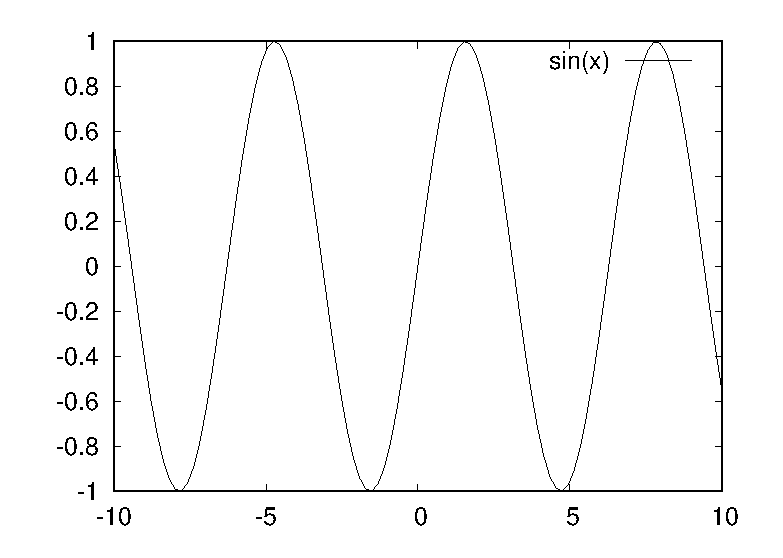
\includegraphics[width=\hsize]{sin.eps}
\caption{正弦関数}
\label{sin}
\end{minipage}
\begin{minipage}[hbtp]{0.49\textwidth}
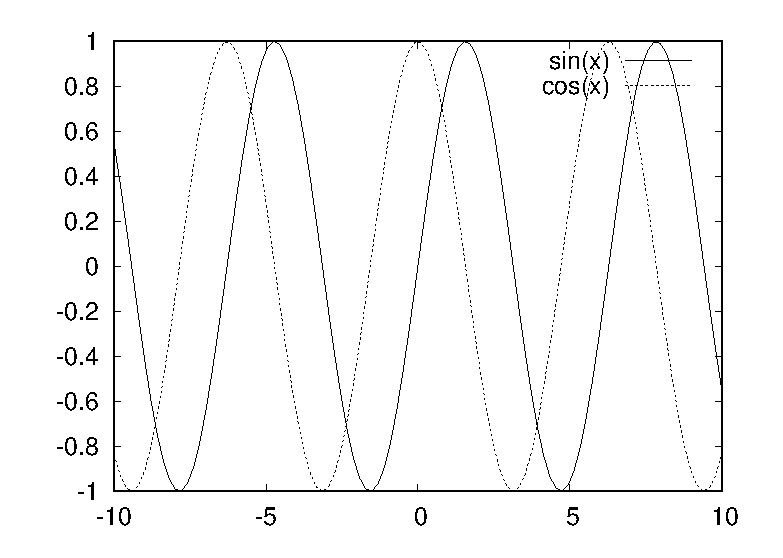
\includegraphics[width=\hsize]{sincos.eps}
\caption{正弦関数と余弦関数}
\label{sincos}
\end{minipage}
\end{figure}

既に作図したグラフに更にグラフを重ねる場合には{\tt\bf replot} を
用います(図\ref{sincos2})。
\begin{terminal}
gnuplot> {\bf replot} cos(x*2)
\end{terminal}

単に {\tt\bf plot cos(x*2)} と入力すると先のグラフが消えてしまうので
注意して下さい。

\begin{figure}
\begin{minipage}[hbtp]{0.49\textwidth}
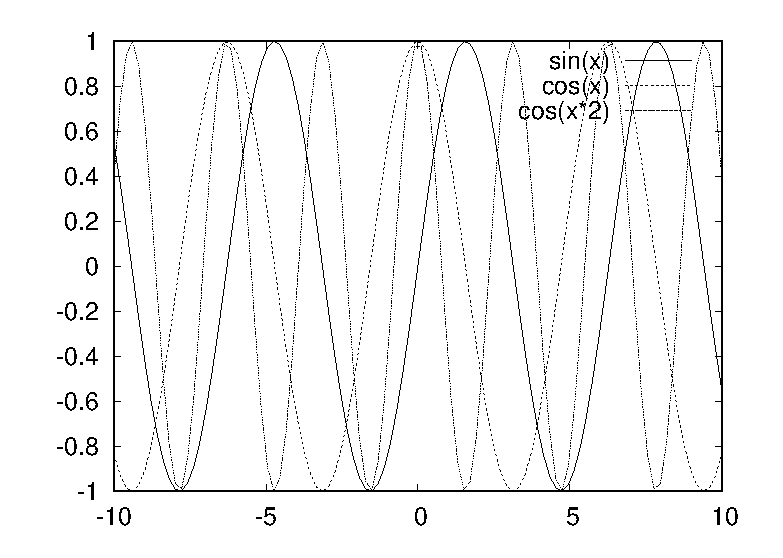
\includegraphics[width=\hsize]{sincos2.eps}
\caption{図\ref{sincos}に $\cos(x*2)$ を重ねた}
\label{sincos2}
\end{minipage}
\begin{minipage}[hbtp]{0.49\textwidth}
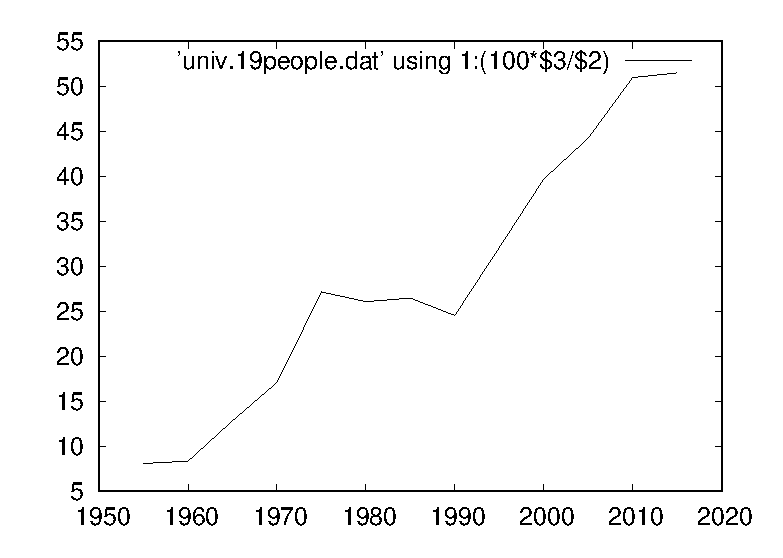
\includegraphics[width=\hsize]{univ.19people1.eps}
\caption{大学入学者数の18歳人口に対する比率}
\label{ratio}
\end{minipage}
\end{figure}

\section{ファイルからデータを読み込む({\tt\bf using, every})}
グラフを表示したいのは形がわかっている関数ばかりではありません。
ファイルに保存してあるデータを読み込んでそれをグラフにする時も
当然あるでしょう。これにもやはり {\tt\bf plot} コマンドを用います。
\begin{terminal}
gnuplot> {\bf plot} 'データファイルの名前'
\end{terminal}
のように、データファイルの名前(絶対パスor相対パス)を ' または '' でくくってやります。
データファイルは一つ以上のスペースで区切られた $(x,y(,z...))$ の
組が複数行から成るものとします。何か適当なデータファイルを作って
それをグラフにしてみましょう。この時、{\tt \#} を含む行の{\tt \#} 以降は
グラフには反映されません。後で見た時にそれが何のデータだったのか
わかるような解説を書いておくと良いでしょう。例えばこんな感じです。
\begin{quote}
 \renewcommand{\arraystretch}{0.7}
\begin{tabular}{lcccc}
{\tt \#} & 大学入学人数 & & & \\
{\tt \#} & (千人) & & & \\
{\tt \#} & 年 & 18歳人口 & 入学者人数\\
&  1955 & 1,682 & 136 \\
&  1960 & 1,998 & 167 \\
&  1965 & 1.948 & 250 \\
&  1970 & 1,947 & 333 \\
&  1975 & 1,561 & 424 \\
&  1980 & 1,580 & 412 \\
&  1985 & 1,556 & 412 \\
&  1990 & 2,005 & 492 \\
&  1995 & 1,773 & 569 \\
&  2000 & 1,511 & 600 \\
&  2005 & 1,365 & 604 \\
&  2010 & 1,214 & 619 \\
&  2015 & 1,200 & 618 \\
\end{tabular}
\end{quote}

このデータはdoverの /home2/masuda2019/enshu2020/data/univ.19people.dat に書いてあります。ファイルから読み込んだデータをプロットする場合、スタイルは {\bf\tt
points} になります。これを変更する場合には
\begin{terminal}
gnuplot> {\bf set style data lines}
\end{terminal}
のように設定しておくか、もしくは
\begin{terminal}
gnuplot> {\bf plot} 'univ.19people.dat' {\bf with line}
\end{terminal}
のように、毎回スタイルを指定します\footnote{スタイルとして {\bf\tt
lines(points)} を設定した場合でも、データファイルが空行(何も書かれて
いない行)を含んでいると、空行の直前のデータと直後のデータの間には
線は引かれません。}。


データファイルに書かれているデータが複数列ある時には、{\tt\bf
plot} コマンドの際に {\tt\bf using} という引数を付けることによって
何列目のデータをグラフにするのかを指定できます。例えば 3 列目の
データを $x$ 軸、1 列目のデータを $y$ 軸にとってグラフを描く場合には
\begin{terminal}
gnuplot> {\bf plot} 'univ.19people.dat' {\bf using 3:1}
\end{terminal}
のようにします。データが 3 列以上ある場合に {\tt\bf using} を省略すると、
1 列目が $x$ 軸、2 列目が $y$ 軸とみなされます。

\vspace*{1zw}
また、 {\tt\bf using} はそれぞれのデータの各列に対応した値を
列番号に {\tt\bf \$}をつけて表すことができます。
例えば1列目のデータは {\tt\bf \$1}、2列目のデータは {\tt\bf \$2}で表さ
れます。
これを利用することによって、各列のデータを{\tt gnuplot}上で演算してグラフに表示させることができます。

また、データファイルの一部だけをプロットしたいときには{\tt\bf every}と
いう引数を用います。例えば、1行おきにプロットする場合には
\begin{terminal}
gnuplot> {\bf plot} 'univ.19people.dat' {\bf every 2}
\end{terminal}
のようにします。

例として、上の「18歳人口と大学入学人数」のデータにおいて
2行目(18歳人口)と3行目(入学者数)の
演算で「大学入学者数の18歳人口に対する比率」という値をグラフ表示させることができます(図\ref{ratio})。
この場合の書式は次のようになります
({\tt\bf p}は{\tt\bf plot}の、{\tt\bf w l}は{\tt\bf with lines}の省略形)。

\begin{terminal}
gnuplot> {\bf p} 'univ.19people.dat' {\bf using 1:(100*{\tt \$}3/{\tt \$}2) w l}
\end{terminal}

\begin{figure}
\begin{center}
\begin{minipage}[hbtp]{0.49\textwidth}
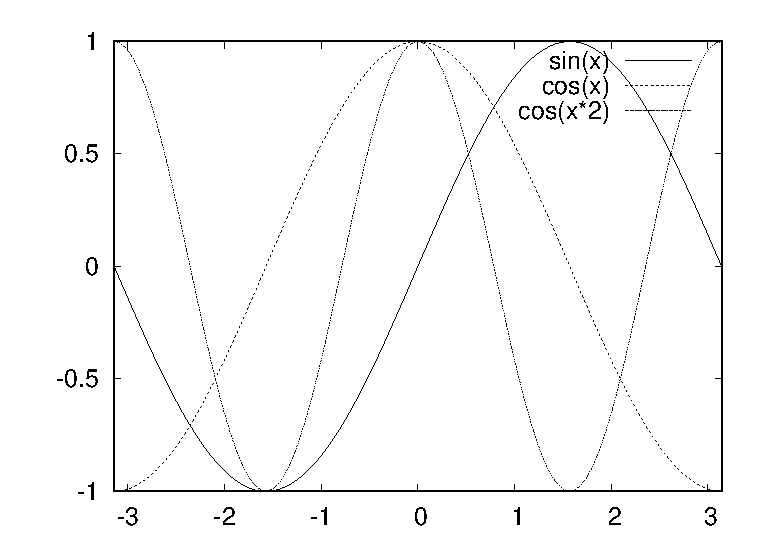
\includegraphics[width=\hsize]{sincos2pi.eps}
\caption{描図範囲を $-\pi$ から $\pi$ までとした}
\label{sincos2pi}
\end{minipage}
\end{center}
\end{figure}

\section{細かい図の指定}
plotコマンドを用いてグラフを書けるようになりましたが、必ずしも自動で設定されるプロット領域と自分の見たい変域が一致しているとは限りません。また、水平軸・鉛直軸が何なのかを明示していない点で情報がまだ不十分です。これらの指定方法について学習しましょう。

\subsection{作図範囲を指定する({\tt\bf set x(y)range, set auto scale})}
作図範囲を指定するには{\tt\bf set xrange} (または {\tt\bf yrange})
コマンドを用います。例えば、$x$ の作図範囲を $-\pi$ から $\pi$ までに
したい時には
\begin{terminal}
gnuplot> {\bf set xrange [-pi:pi]}
\end{terminal}
と入力します。ただし{\tt\bf set} コマンドは設定を変えるだけですから、
画面に表示されているグラフは変化しません。画面に表示されているグラフを
更新するには
\begin{terminal}
gnuplot> {\bf replot}
\end{terminal}
と入力してもう一度作図し直す必要があります(図\ref{sincos2pi})。
$y$ に関する作図範囲も同様に {\tt\bf set yrange} コマンドに
よって変えられます。

作図範囲の指定を取り消したい場合には
\begin{terminal}
gnuplot> {\bf set autoscale}
\end{terminal}
と入力します。もちろんこの後にも {\tt\bf replot} と入力する必要が
あります。以降このテキストでは {\tt\bf replot} の入力は省略しますが、
設定を変えた({\tt\bf set} コマンドを使った)後は必ず {\tt\bf replot} と
入力して図に反映させる必要があります。

\subsection{曲線に名前を付ける({\tt\bf title, set key})}
{\tt\bf plot} コマンドによってグラフを描くと、右上にそれがどういう
曲線か表示されます。これを変えるには{\tt\bf plot} コマンドの
際に {\tt\bf title} という引数を加えます(図\ref{hogehoge})。
\begin{terminal}
gnuplot> {\bf plot} sin(x) {\bf title} 'hogehoge'
\end{terminal}
曲線の名前の部分を ' または '' でくくることに注意して下さい。

曲線の名前を表示する必要がない時には
\begin{terminal}
gnuplot> {\bf plot} sin(x) {\bf title} 'hogehoge', sin(x)%
*cos(x) notitle
\end{terminal}
のようにします(図\ref{hogehoge2})。

曲線の名前の表示場所を設定するには{\tt\bf set key} というコマンドを
使います。ここでは詳しい説明は省略しますので、オンラインマニュアルで
その使い方を確かめてみて下さい。

\begin{figure}
\begin{minipage}[hbtp]{0.49\textwidth}
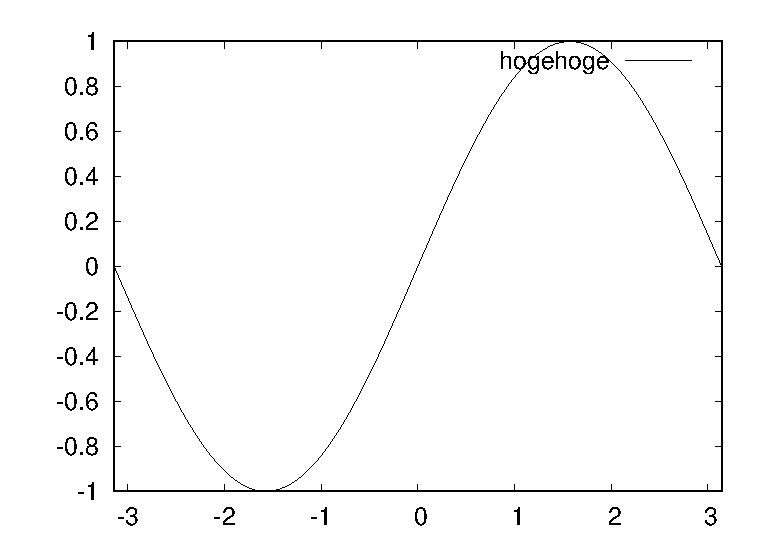
\includegraphics[width=\hsize]{hogehoge.eps}
\caption{曲線に名前をつける}
\label{hogehoge}
\end{minipage}
\begin{minipage}[htbp]{0.49\textwidth}
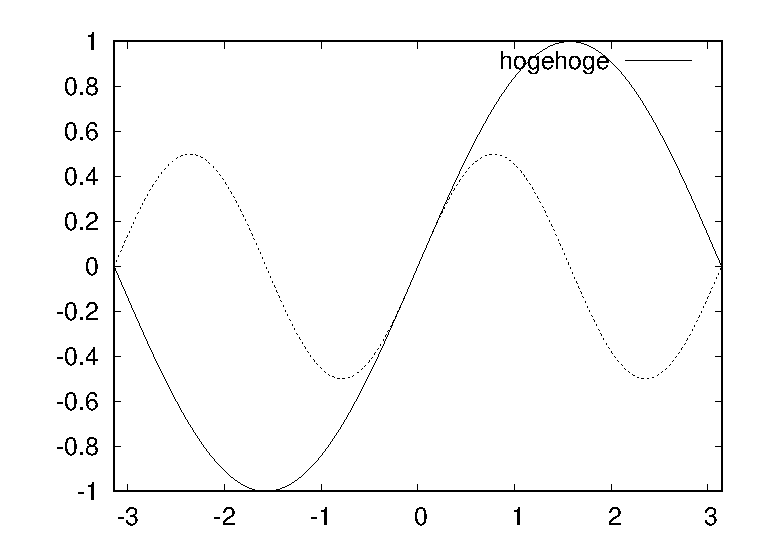
\includegraphics[width=\hsize]{hogehoge2.eps}
\caption{図\ref{hogehoge}に無名の曲線を重ねた}
\label{hogehoge2}
\end{minipage}
\end{figure}

\subsection{描写スタイルを変える({\tt\bf set style function, with, set grid})}
今まで表示したグラフは連続した曲線で描かれていました。この表示方法を
変えるコマンドとして{\tt\bf set style function} があります。例えば
\begin{terminal}
gnuplot> {\bf set style function steps}
\end{terminal}
としてみましょう。グラフが階段状になりましたね(図\ref{steps})。

\begin{figure}
\begin{minipage}[hbtp]{0.49\textwidth}
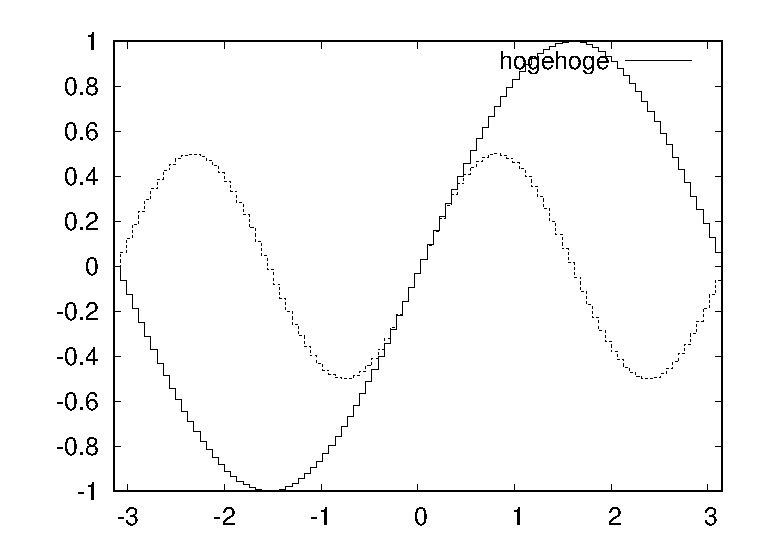
\includegraphics[width=\hsize]{steps.eps}
\caption{図\ref{hogehoge2}の表示スタイルを {\tt\bf steps} にした}
\label{steps}
\end{minipage}
\begin{minipage}[hbtp]{0.49\textwidth}
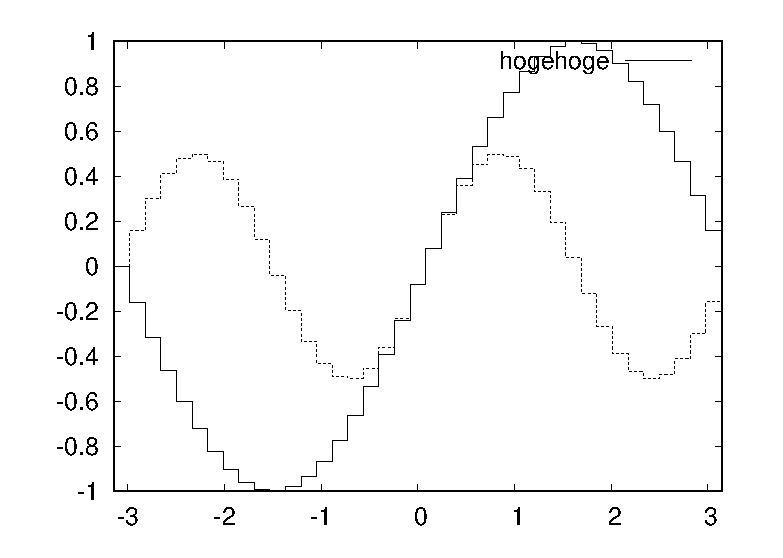
\includegraphics[width=\hsize]{steps40.eps}
\caption{図\ref{steps}の段の数を 40 段にした場合}
\label{steps40}
\end{minipage}
\end{figure}

段の数(一般にはgnuplotが描画のためにサンプルする点数)を変えるには{\tt\bf set samples} というコマンドを用います。
\begin{terminal}
gnuplot> {\bf set samples 40}
\end{terminal}
とすれば、40 段のグラフが描かれます(図\ref{steps40})。

グラフの表示はこの他にも、点線({\tt\bf dots})や棒グラフ({\tt\bf boxes})、
パルス状のグラフ({\tt\bf impulses})などが使えます。詳しくは、
\begin{terminal}
gnuplot> {\bf help set style}
\end{terminal}
を見てください。

複数のグラフをそれぞれ異なったスタイルで描きたい場合には、
{\tt\bf plot} コマンドの際に {\tt\bf with} をつけて指定します。例えば
\begin{terminal}
gnuplot> {\bf plot} sin(x) {\bf with points}, sin(x)%
*cos(x) {\bf with impulses}
\end{terminal}
のようにします(図\ref{with})。

{\tt\bf set grid} コマンドを使うと、$x$ 軸、$y$ 軸それぞれの目盛が
刻まれている値の格子が入ります(図\ref{grid})。格子を消すには {\tt\bf unset grid} とします。

\begin{figure}
\begin{minipage}[hbtp]{0.49\textwidth}
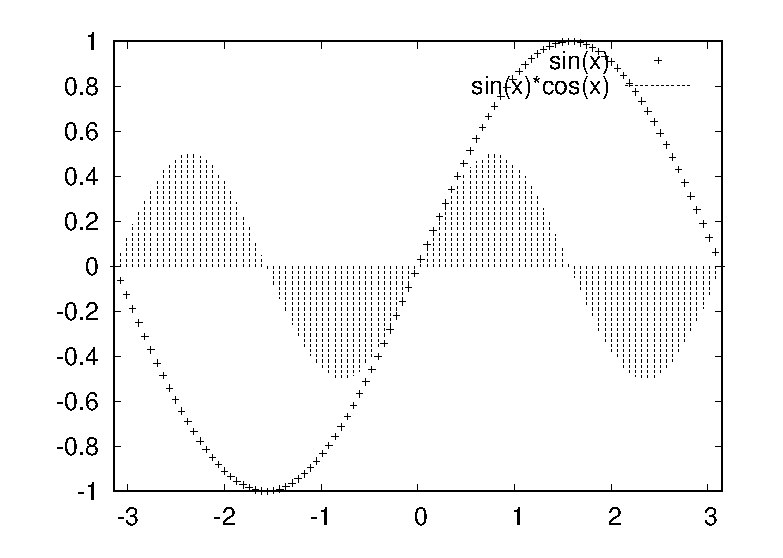
\includegraphics[width=\hsize]{with.eps}
\caption{{\tt\bf points} と {\tt\bf impulses} のグラフの例}
\label{with}
\end{minipage}
\begin{minipage}[hbtp]{0.49\textwidth}
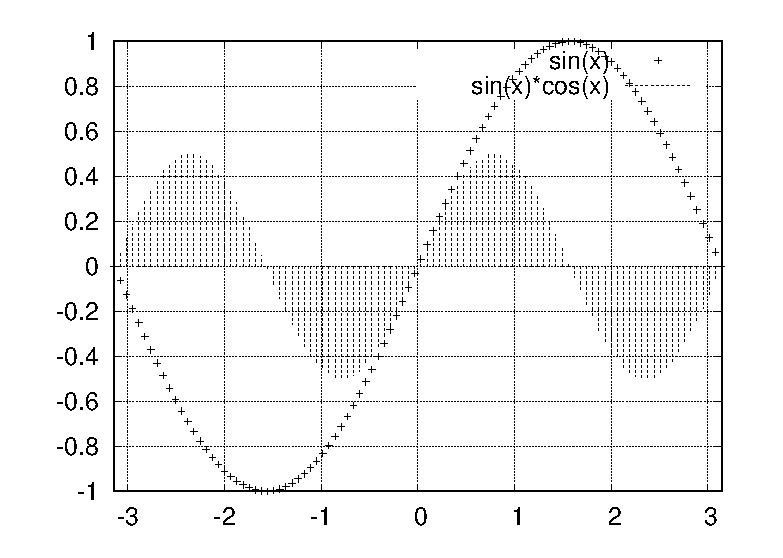
\includegraphics[width=\hsize]{grid.eps}
\caption{図\ref{with}に格子をいれた}
\label{grid}
\end{minipage}
\end{figure}

\subsection{対数プロット({\tt\bf set logscale})}
gnuplot では対数軸の作図も可能です。例えば
\begin{terminal}
gnuplot> {\bf set logscale y} \\
gnuplot> {\bf plot} exp(x+1)
\end{terminal}
としてみましょう。$y$ 軸が対数表示になりましたね(図\ref{exp})。
{\tt\bf logscale} の後を省略した場合には全ての軸が対数軸になります。

対数プロットをやめるには {\tt\bf unset logscale y} とします。

\begin{figure}
\begin{center}
\begin{minipage}[hbtp]{0.49\textwidth}
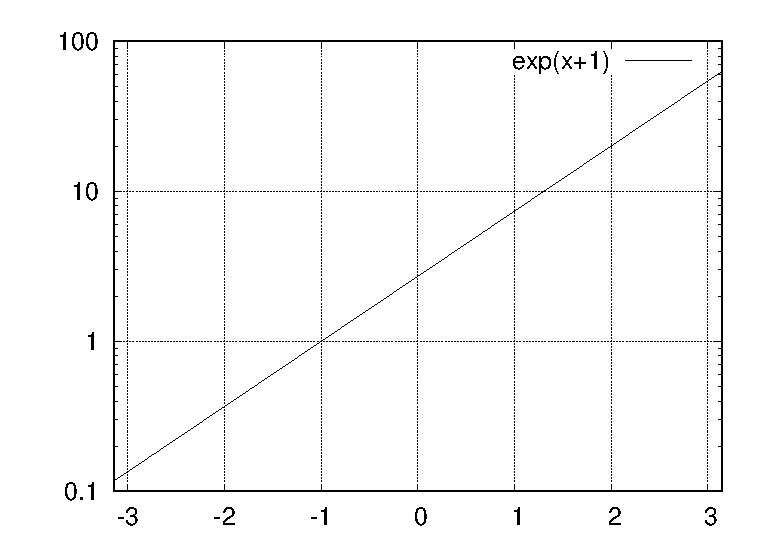
\includegraphics[width=\hsize]{exp.eps}
\caption{片対数グラフの例}
\label{exp}
\end{minipage}
\end{center}
\end{figure}


\subsection{軸に名前をつける({\tt\bf set x(y)label, title})}
大学入学者数のデータを例として、$x$ 軸と $y$ 軸が何を意味して
いるのか表示させてみましょう。これには {\tt\bf set xlabel} (または {\tt\bf
ylabel})を用います(図\ref{label})。
\begin{terminal}
{\tt gnuplot> {\bf set xlabel 'year'}} \\
{\tt gnuplot> {\bf set ylabel 'new students / 18-year-old (\%)'}}
\end{terminal}
グラフ全体の表題を付けるには {\tt\bf set title} です。
\begin{terminal}
gnuplot> {\bf set title 'New University Students in Japan'}
\end{terminal}

\subsection{軸の目盛をかえる({\tt\bf set x(y)tics})}\label{ticsec}
データファイルで使っている単位と、描きたいグラフの単位が異なって
いることはよくあることです。このような場合には {\tt\bf set
xtics} (または {\tt\bf ytics}) コマンドを使って目盛の振り方を変更
します。
'univ.19people.dat'の1列目は西暦表示となっていますが、 これを元号に直すには以下のようにします。
\begin{terminal}
gnuplot> {\bf set xtics('S25' 1950,\ ' ' 1955,\  'S35' 1960,\ ' ' 1965,\ 'S45' 1970,\ ' ' 1975,\ 'S55' 1980,\ ' ' 1985,\  'H02' 1990,\ ' ' 1995,\ 'H12' 2000,\ ' ' 2005,\  'H22' 2010,\ ' ' 2015,\ 'R2' 2020)}
\end{terminal}
これで、1950, 1960, 1970, 1980, 1990, 2000, 2010, 2020 の位置にはそれぞれ S25, S35, S45, S55, H02, H12, H22, R2 という目盛が振られ、1955, 1965, 1975, 1985, 1995, 2005, 2015 の位置には何も書かれていない目盛が刻まれます(図\ref{tics})。
$y$ 軸に目盛を入れる場合も同様です。

また、目盛りの値には元ファイルの値を用いつつ目盛りの間隔を変更したい場合には、{\tt\bf set xtics <刻み幅>}とします。 引数なしに単に {\tt\bf set xtics} とした場合には、目盛は標準 (自動指定)のものに戻ります。目盛が不要の場合には {\tt\bf unset tics} と します。また、{\tt\bf xtics font "フォント名,フォントサイズ"}とすればフォントサイズや種類を変えることができます。デフォルトのフォントサイズは小さめなので、スライド用のグラフを作成するときなどはこれを使用して目盛を読み取りやすくしましょう。普段は表示されていませんが小目盛の設定もでき、{\tt\bf mxtics <分割数>}とすると小目盛の数を変更できます。

\begin{figure}
\begin{minipage}[hbtp]{0.49\textwidth}
\begin{center}
% \includegraphics[width=\textwidth]{Graphics/univ.18people2.eps}
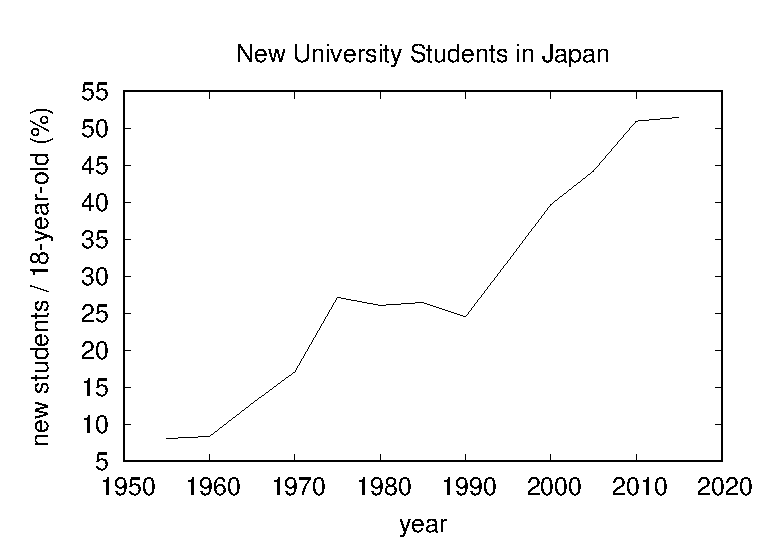
\includegraphics[width=\hsize]{univ.19people2.eps}
\caption{各タイトルを入れた例}
\label{label}
\end{center}
\end{minipage}
\begin{minipage}[hbtp]{0.49\textwidth}
\begin{center}
% \includegraphics[width=\textwidth]{Graphics/univ.18people3.eps}
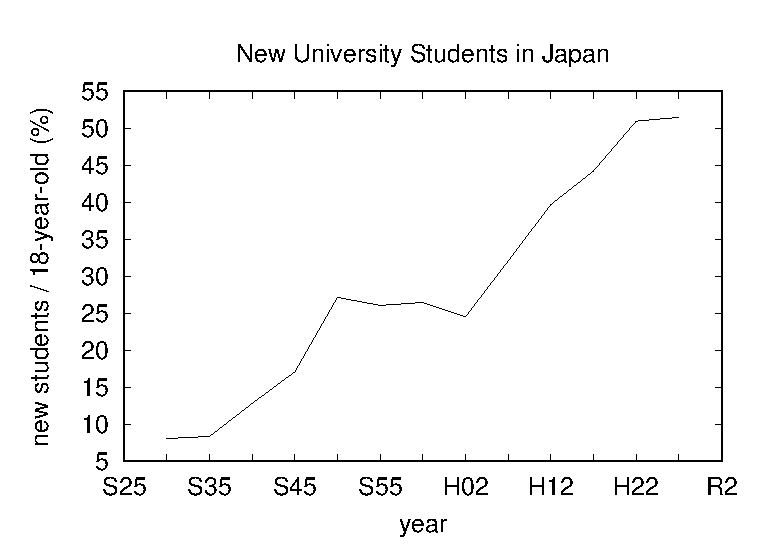
\includegraphics[width=\hsize]{univ.19people3.eps}
\caption{図\ref{label}の目盛を和暦にした例}
\label{tics}
\end{center}
\end{minipage}
\end{figure}

\section{エラーバーを付ける({\tt\bf errorbars})}
観測値や実験値をグラフにする場合の多くは、そこにエラーバーを表示する
必要があります。このような場合には {\tt\bf errorbars} というスタイルを
指定します。
\begin{terminal}
gnuplot> {\bf set style data errorbars}
\end{terminal}
または
\begin{terminal}
gnuplot> {\bf plot} 'observation.dat' {\bf with errorbars}
\end{terminal}

データファイルには、3 列または 4 列のデータが必要です。データが 3 列の
場合にはそれぞれの行は $(x,y,\Delta y)$ の組として解釈され、
$(x,y$-$\Delta y)$ から $(x,y$+$\Delta y)$ までの線が引かれます。
データが 4 列の場合には、それそれの列は $(x,y,y{\rm low},y{\rm high})$ と
して解釈され、$(x,y{\rm low})$ から $(x,y{\rm high})$ までの線が
引かれます。複数列のデータの中から使用する列を指定する場合には、次の
ように {\tt\bf using} を使います。
\begin{terminal}
gnuplot> {\bf plot} 'observation.dat' {\bf using 1:4:3:5 with errorbars}
\end{terminal}
%
%{\tt\bf errorbars} を指定した場合には、データの各点を結ぶ線は描かれ
%ません。

\section{練習問題 1}
先に進む前に、ここまで学習したことの確認をしましょう。
\begin{enumerate}
\item
     doverの /home2/masuda2019/enshu2020/data/univ.19people.dat をscpで手元に持ってくる。
\item
     横軸に西暦、縦軸に大学新入生数をプロットする。
\item
     横軸に西暦、縦軸に18歳人口をとって棒グラフでプロットする。(ヒント:{\tt\bf
     with boxes})
\item
     横軸に和暦、縦軸に18歳人口に対する大学新入生数の割合をプロットする。
\item
     前問のグラフに縦軸と横軸にラベルをつけ、タイトルもつける。\\
\end{enumerate}

\section{plt ファイルと load({\tt\bf load '***.plt'})}
ここまではすべて対話方式でコマンドを入力してきましたが、
複数のコマンドをひとつのファイルに書いて
まとめて一気に実行することができます。
コマンドファイルには、例えば以下の 'univ.19people.plt' のように、
一般に plt という拡張子を用いる場合が多いです。
Emacs等のエディタで以下の内容のファイルを書いてみてください。

\begin{terminal}
 set xlabel 'year'\\
 set ylabel 'new students / 18-year-old (\%)'\\
 set title 'New University Students in Japan'\\
 set xtics('S25' 1950,' ' 1955, 'S35' 1960,' ' 1965,'S45' 1970,' ' 1975,'S55' 1980,' ' 1985, 'H02' 1990,' ' 1995,'H12' 2000,' ' 2005, 'H22' 2010, ' ' 2015, 'R2' 2020)\\
 set xrange [1950:2020]\\
 set yrange [0:60]\\
 set ytics 10\\
 p 'univ.19people.dat' using 1:(100*\$3/\$2) w l
\end{terminal}

これらのコマンド群を一気に実行するには{\tt\bf load}というコマンドを
使います。

\begin{terminal}
gnuplot> {\bf load 'univ.19people.plt'}
\end{terminal}

としてみると練習問題1の図が作れます。

\section{3次元プロット}
gnuplotでは3次元のグラフも作成することができます。
\subsection{3 次元プロット({\tt\bf splot, set view})}
3 次元プロットする際には {\tt\bf splot} というコマンドを使います。
\begin{terminal}
gnuplot> {\bf splot} sin(x/5)*cos(y/5)
\end{terminal}
デフォルトでは視点の位置は $x$ 軸から $60^{\circ}$、 $z$ 軸から 
$30^{\circ}$ の地点になります(図\ref{splot})。これを変更するには {\tt\bf
set view} コマンドを用います(図\ref{view})。
\begin{terminal}
gnuplot> {\bf set view 50,60}
\end{terminal}
とすれば、画面水平右向きが $x$ 軸、鉛直上向きが $y$ 軸、画面手前
向きが $z$ 軸であった座標系を、$x$ 軸の周りに $50^{\circ}$ $z$ 軸の
周りに $60^{\circ}$ それぞれ回転させたグラフの画面への投射像が
得られます。
また、最近のgnuplotではマウスで図を回転させることも可能です。

\begin{figure}
\begin{minipage}[bhtp]{0.49\textwidth}
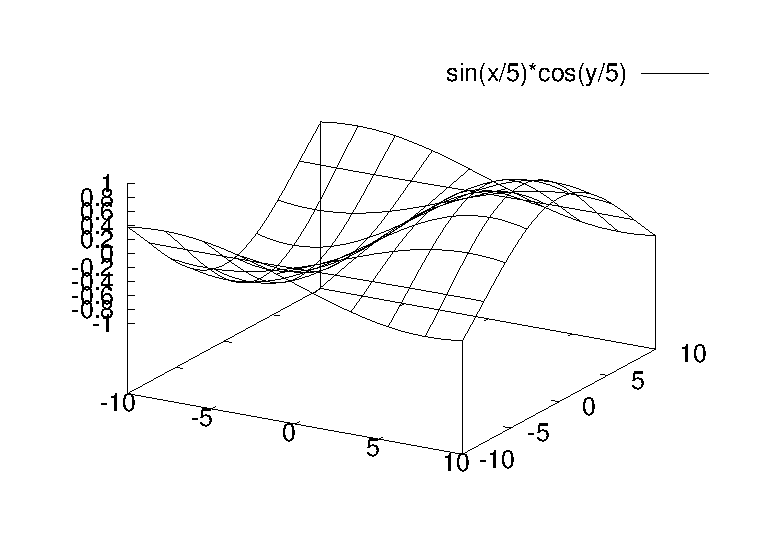
\includegraphics[width=\hsize]{splot.eps}
\caption{3 次元プロットの例}
\label{splot}
\end{minipage}
\begin{minipage}[bhtp]{0.49\textwidth}
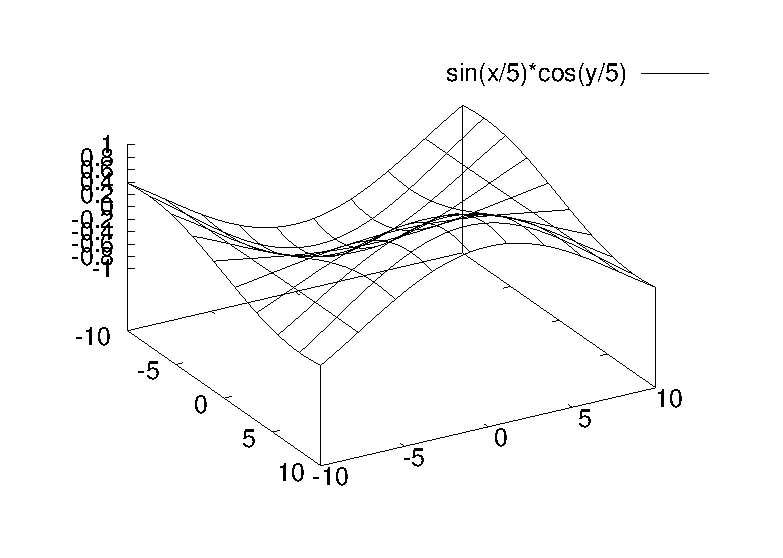
\includegraphics[width=\hsize]{view.eps}
\caption{図\ref{splot}の視点の位置を変更}
\label{view}
\end{minipage}
\end{figure}

データファイルから値を読み込んで 3 次元プロットする際には
{\tt\bf plot} コマンド同様
\begin{terminal}
gnuplot> {\bf splot} 'data3d.dat' {\bf with line}
\end{terminal}
のようにします\footnote{バージョンによっては {\tt\bf splot}の
前に {\tt\bf set parametric} を設定しなければならないかも知れません}。
この時、データファイルには 3 列以上のデータが書かれていることが
必要です\footnote{1 列だけの場合にも 3 次元プロットができます。
{\tt\bf parametric} オンラインマニュアルを参照のこと}。
3次元データは($X,Y,Z$)の組にして与えます。出力形式は以下のようにします。
(\textbf{注意!!空行が一行必要です。})
\begin{quote}
 \renewcommand{\arraystretch}{0.7}
\begin{tabular}{lcccc}
{\tt \#} & x & y & z & \\
&  0 & 0 & 0 \\
&  0 & 1 & 1 \\
&  0 & 2 & 4 \\
&  0 & 3 & 9 \\
\\
&  1 & 0 & 1 \\
&  1 & 1 & 2 \\
&  1 & 2 & 5 \\
&  1 & 3 & 10 \\
\\
&  2 & 0 & 2 \\
&  2 & 1 & 3 \\
&  2 & 2 & 6 \\
&  2 & 3 & 11 \\
\\
&  3 & 0 & 3 \\
&  3 & 1 & 4 \\
&  3 & 2 & 7 \\
&  3 & 3 & 12 \\
\end{tabular}
\end{quote}

ファイルに空行で区切られた同数のデータが複数書かれている場合、
スタイルとして {\tt\bf lines} ({\tt\bf points}) を指定するとデータを
格子上に結んだグラフが描かれます。\\
(上記データはdoverの /home2/masuda2019/enshu2020/data/data3d.dat にあるので
データ形式を確認した上で{\tt\bf splot} してみてください。)

\subsection{コンタープロット({\tt\bf set contour(surface), set contrparam})}
コンタープロットとは等高線地図を描くことです。等高線地図を
描くには 3 次元データをプロットする時に
\begin{terminal}
gnuplot> {\bf set contour}
\end{terminal}
と設定します。すると、$x$-$y$ 平面上に等高線地図が描かれます
(図\ref{contour})。

\begin{figure}
\begin{center}
\begin{minipage}[hbtp]{0.49\textwidth}
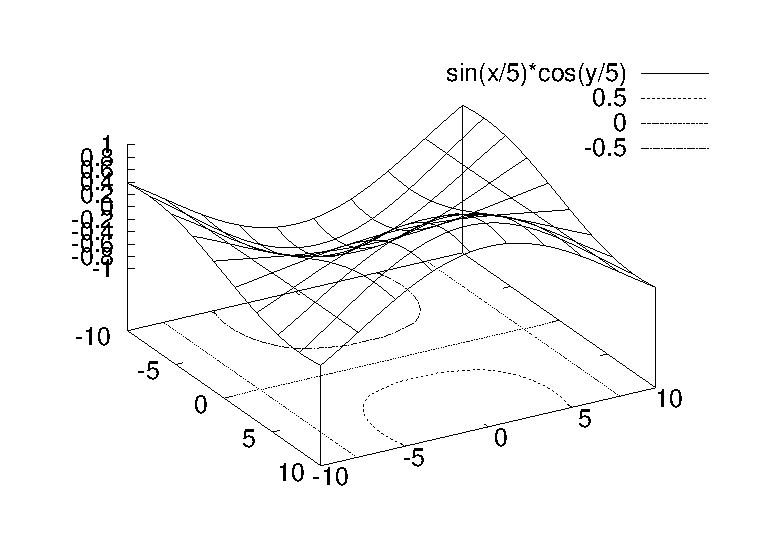
\includegraphics[width=\hsize]{contour.eps}
\caption{図\ref{view}に等高線を描いたもの}
\label{contour}
\end{minipage}
\end{center}
\end{figure}

等高線を $x$-$y$ 平面ではなくグラフの曲面上に重ねるには
\begin{terminal}
gnuplot> {\bf set contour surface}
\end{terminal}
と設定します。

等高線を描く際の様々なパラメタ(等高線を描く際の近似の仕方、等高線の
開始値、幅、終了値等)を変更するには {\tt\bf cntrparam} の値を設定します。
例えば
\begin{terminal}
gnuplot> {\bf set cntrparam levels incremental 0,0.5}
\end{terminal}
とすると、0 から開始して 0.5 刻みで等高線が描かれます。詳しくは
{\tt\bf cntrparam} のオンラインマニュアルを見て下さい。

等高線地図は多くの場合 $x$-$y$ 平面に投影した形で表されます。
そのためには次のような設定をすると良いでしょう。
\begin{terminal}
gnuplot> {\bf unset surface} \\
gnuplot> {\bf set view 0,0} \\
gnuplot> {\bf unset ztics}
\end{terminal}
それぞれのコマンドの意味はオンラインマニュアルで確かめてみて下さい。

ファイルからデータを読みとって等高線地図を描く場合には、データファイルに
欠損値があってはならないことに気をつけて下さい。

\subsection{カラーのグラデーション表示にする({\tt\bf set pm3d})}
三次元の図をカラーのグラデーションにする方法として{\tt\bf pm3d} というものがあります。
\begin{terminal}
gnuplot> {\bf set pm3d}
\end{terminal}
とすると、このあとの三次元プロットはグラデーションを用いたものとなります。
ためしに
\begin{terminal}
gnuplot> {\bf splot} sin(x/5)*cos(y/5)
\end{terminal}
としてみてください。さきほどの図\ref{splot}の時と違ってグラデーションになったでしょうか。\\
ちなみに、このモードをやめるときは
\begin{terminal}
gnuplot> {\bf unset pm3d}
\end{terminal}
とすればもとのモードになります。

同様に $x-y$ 平面に投影された等高線をグラデーションにするには
\begin{terminal}
gnuplot> {\bf set pm3d at b}
\end{terminal}
としてください。図\ref{contour}の場合と比較するために、
\begin{terminal}
gnuplot> {\bf unset surface}\\
 gnuplot> {\bf set view 0,0} \\
 gnuplot> {\bf unset ztics} \\
 gnuplot> {\bf splot} sin(x/5)*cos(y/5)
\end{terminal}
としてみましょう。

\section{複数のグラフを描写する({\tt\bf set multiplot})}
一度に複数のグラフを描写する場合には {\tt\bf set multiplot} コマンドを
使います。このコマンドにより gnuplot は {\tt\bf multiplot} のモードに
入ります。例えば
\begin{terminal}
gnuplot> {\bf set multiplot} \\
multiplot> {\bf set size 1,0.5} \\
multiplot> {\bf set origin 0,0.5} \\
 multiplot> {\bf plot} sin(x) \\
 multiplot> {\bf set origin 0,0} \\
 multiplot> {\bf plot} cos(x)
\end{terminal}
とすると、上に $\sin x$ 下に $\cos x$ のグラフが描かれます(図\ref{multi})。
{\tt\bf set origin} コマンドはグラフの左下の位置を決め、
{\tt\bf set size} コマンドはグラフの縦横のサイズを変更します。

\begin{figure}
\begin{center}
\begin{minipage}[hbtp]{0.49\textwidth}
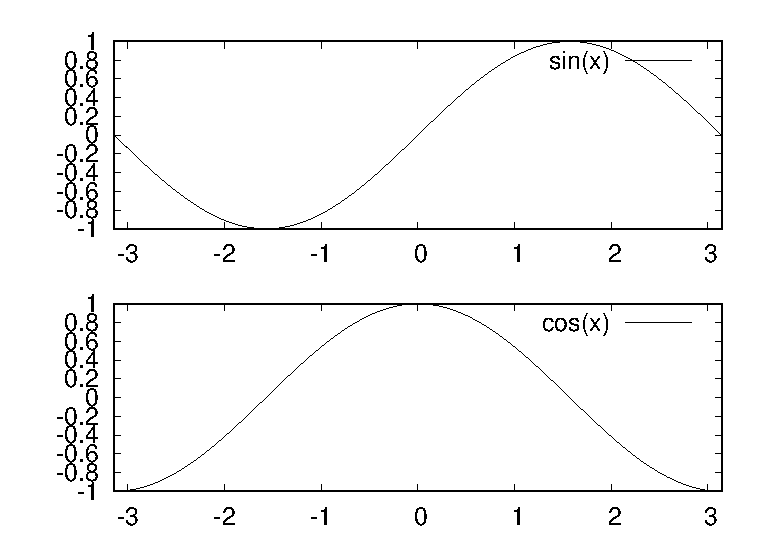
\includegraphics[width=\hsize]{multi.eps}
\caption{2つのグラフを一度に描写}
\label{multi}
\end{minipage}
\end{center}
\end{figure}

{\bf\tt multiplot} モードを終了させるには
\begin{terminal}
multiplot> {\bf unset multiplot}
\end{terminal}
と入力して下さい。

\section{グラフを出力する({\tt\bf set terminal postscript, set output})}
グラフを印刷するためには、画面の情報をポストスクリプト形式でファイルに保存する必要があります。これには次のようにします。
\begin{terminal}
 gnuplot> {\bf set terminal postscript} \\
 gnuplot> {\bf set output 'output.ps'} \\
 gnuplot> {\bf replot}
\end{terminal}
出力先を決めた後に {\tt\bf replot} をすることを忘れないでください。
terminalをファイル出力に変えてからグラフを書き出さなければ
何も書かれません。
{\tt\bf replot}とすると直前のプロットと同じものを書き出すことができます。

出力ファイルを閉じるには、
\begin{terminal}
 gnuplot> {\bf set output}
\end{terminal}
とします。
(\textbf{注意!!{\tt\bf set output}をしないで他へ出力に切
り替える({\tt\bf set terminal qt}等)とファイルが壊れるので、
ファイルを閉じるか、gnuplotを一度終了する({\tt\bf quit})のを忘
れないようにしてください。})

また、このままの状態だとプロット出力が postscript に書かれるので、
出力を再び画面に表示するために
\begin{terminal}
 gnuplot> {\bf set terminal qt}
\end{terminal}
とします。

出来上がった図は{\tt\bf gv}というコマンド (PostScript and PDF view) で見ることができます。
\begin{terminal}
{\bf gv output.ps}
\end{terminal}

また、デフォルトでは
グラフは横描き({\it landscape})に出力されるのですが、これを
縦描き({\it portrait})にしたい場合には
\begin{terminal}
 gnuplot> {\bf set terminal postscript portrait}
\end{terminal}
のように設定します。また
\begin{terminal}
 gnuplot> {\bf set size 0.5,0.25}
\end{terminal}
と設定すると、グラフが横に半分、縦に 1/4 の大きさになります。
図の縦横比を変更したいときは
\begin{terminal}
 gnuplot> {\bf set size ratio 2.0}
\end{terminal}
とすると、縦:横=2:1の図を作ることができます。

{\tt \bf set terminal}はpostscript形式に限らず様々な形式で出力できま
す。
例えば、描画ソフトであるTgifのファイル形式で出力するときには、以下のようにします。
\begin{terminal}
 gnuplot> {\bf set terminal tgif} \\
 gnuplot> {\bf set output 'output.obj'} \\
 gnuplot> {\bf replot}
\end{terminal}

要はterminalの種類をtgifと指定するだけです。

同様にして、作成した図をLatexに貼りつける際にはeps (Encapsulated Postscript)形式で
出力する必要があります。その場合には
\begin{terminal}
 gnuplot> {\bf set terminal postscript eps}
\end{terminal}
のようにします。カラーで出力したい場合には
\begin{terminal}
 gnuplot> {\bf set terminal postscript eps color}
\end{terminal}
などとしてください。eps や color などのオプションは、
\begin{terminal}
 gnuplot> {\bf help set terminal postscript}
\end{terminal}
とすることで調べることができます。

tgif や eps ファイル以外にも、png、jpg、ps、pdf等、様々な
ファイル形式に書き出すことができます。
詳しくは、
\begin{terminal}
 gnuplot> {\bf help set terminal}
\end{terminal}
で調べてみて下さい。
また、これらの画像ファイルを表示するには{\tt\bf display}(ImageMagick)というコマンド
が便利です。

\section{load と save}
先ほど{\tt\bf load} というコマンドを学びましたが、
この{\tt\bf load} と兄弟関係にあるコマンドが {\tt\bf save} です。
{\tt\bf save}コマンドを用いることで、
これまでに対話形式で実行してきたコマンドを
先程自分で書いた plt ファイルと同様な出力として得られます。\\
例えば、
\begin{terminal}
 gnuplot> {\bf p cos(x)} \\
 gnuplot> {\bf set xlabel 'x'} \\
 gnuplot> {\bf set ylabel 'y'}\\
 gnuplot> {\bf set terminal postscript}\\
 gnuplot> {\bf set output 'cos.ps'}\\
 gnuplot> {\bf rep}\\
 gnuplot> {\bf save 'cos.plt'}
\end{terminal}
としてみましょう({\tt\bf rep}は{\tt\bf replot}の省略形)。\\
これをemacsなどで開いてみると、\\
----- ここから ----- ここから ----- ここから ----- ここから -----
\begin{verbatim}
#!/usr/bin/gnuplot -persist
#
#    
#    	G N U P L O T
#    	Version 4.6 patchlevel 6    last modified September 2014
#    	Build System: Linux i686
#    
#    	Copyright (C) 1986-1993, 1998, 2004, 2007-2014
#    	Thomas Williams, Colin Kelley and many others
#    
#    	gnuplot home:     http://www.gnuplot.info
#    	faq, bugs, etc:   type "help FAQ"
#    	immediate help:   type "help"  (plot window: hit 'h')
# set terminal postscript landscape noenhanced defaultplex \
   leveldefault monochrome colortext \
   dashed dashlength 1.0 linewidth 1.0 butt noclip \
   nobackground \
   palfuncparam 2000,0.003 \
   "Helvetica" 14  fontscale 1.0 
# set output 'cos.ps'
\end{verbatim}
\hspace{2cm} \vdots
\begin{verbatim}
set loadpath 
set fontpath 
set psdir
set fit noerrorvariables noprescale
GNUTERM = "x11"
p cos(x)
#    EOF
----- ここまで ----- ここまで ----- ここまで ----- ここまで -----
\end{verbatim}
のように書かれていると思います。\\
一瞬意味不明に見えるかも知れませんが、これは実際に{\tt gnuplot>} において入力することができるコマンドを並べた
 だけなのです。 自分で打ち込んでない部分(例えばここでは、{\tt \bf set loadpath}な
 ど)は、gnuplotが勝手に解釈してデフォルトの環境を出力してくれます。この
 ファイルを良く見ると、自分で入力した{\tt \bf set title}や{\tt \bf set
 xlabel}が書き出されていることが分かると思います。{\tt \bf p cos(x)}は設定された環境が全て反
 映されるように最後に書かれるようになっ ています。\\
このファイルを先ほど学んだ{\tt\bf load}コマンドで読み込めば同じ状況が
再現されます。ただし、{\tt\bf set terminal postscript}や{\tt\bf set
output 'cos.ps'}のように、terminalのタイプを変更したり何かを出力し
たりするコマンドの部分は、{\tt\bf save}で出力したコマンドファイルではコ
メントアウトされます。皆さんのファイルでもきっとそうなっていることと思い
ます(コマンドファイルのコメントアウトの最後の部分)。もしloadすることで
postscriptファイルを作りたければ、この部分のコメントアウトを消したうえで
、先ほど学んだ{\tt\bf load}コマンドを用いるかあるいはktermなど普通のター
ミナル上で
\begin{terminal}
\$ gnuplot cos.plt
\end{terminal}
と入力することでpostscriptファイルを作ってやることができます。

plt ファイルはこれから研究をする上でとても強力な手段となります。
例えば$\sin{x},\sin{2x},\sin{3x}$のグラフを出力し
たいとします。この時、いちいちgnuplotを立ち上げて何度も{\tt \bf plot
sin(x)}などと打つのは面倒ですよね(まあ、3つぐらいなら面倒ではないかも知れま
せんが、$\sin{100 x}$までだとしたらどうでしょう)。そんな時は、前もっ
てemacsなどで
\begin{verbatim}
----- ここから ----- ここから ----- ここから ----- ここから -----
#! /usr/bin/gnuplot
set xrange [0:2*pi]
set yrange [-1:1]
set terminal postscript
set output "sin1x.ps"
p sin(x)
set output "sin2x.ps"
p sin(2*x)
set output "sin3x.ps"
p sin(3*x)
----- ここまで ----- ここまで ----- ここまで ----- ここまで -----
\end{verbatim}
と書いておきます。コピー\&ペースト等を使えば簡単ですね。たとえば
sintest.pltという名前で保存したとします。その上で、
\begin{terminal}
\$ gnuplot sintest.plt
\end{terminal}
とすると…、一発で3つのpostscriptファイルができてしまいます!!\\
後から学ぶと思いますが、unixのコマンドを用いれば、$\sin{x}$から$\sin{100x}$まで出力するようなコ
マンドファイルだって簡単に作れてしまいます。unix(シェル)とコマンドファイ
ルのコンビネーションによって、gnuplotは非常に強力なアイテムになります。
\\
「そんなことしないよ。」と思っている人がいるかもしれません。しかし、研究をしていく上でこう
いったことは意外と良くあります。例えば、「数値計算を行って10秒ごとにデータを取り、それを全てグラフにして時間発展を見たい!」と
思った時にこの技が大変役に立ちます。\\\\
%P.S. もちろん、コマンドファイルは{\tt\bf set terminal postscript}などとせず、ただ
%{\tt \bf plot,replot}をするだけにも使えます。

\section{練習問題 2}
\begin{enumerate}
\item
     $f(x,y) = x^2 \exp \left(-x^2\right) y^2 \exp \left(-y^2\right)$
     を $-3<x<3$, $-3<y<3$
     の範囲で3次元プロット ({\tt\bf splot})する。
\item
     メッシュの数を増やす。(ヒント:{\tt\bf set isosample })
\item
     等高線を底面に描く。
\item
     pm3dを用いてカラーのグラデーションを用いてプロットしてみる。
\item
     load すると一発で $f(x,y)$
     を $-3<x<3$, $-3<y<3$ の範囲で
     底面だけを2次元表示する plt ファイル
     をゼロから自分で書く。(ヒント:{\tt\bf set pm3d map})
\item
     eps形式かつカラー表示で書きだし、gvで図ができていることを確認する。\\
     →課題2へ。
\end{enumerate}

\newpage
\section*{Appendix 1:  アニメーション}
先ほどのコマンドファイルをうまく使うと、アニメーションを作ってやることが
できます。\\
たとえば…、
\begin{verbatim}
----- ここから ----- ここから ----- ここから ----- ここから -----
#! /usr/bin/gnuplot
set xrange [-20:20]
set yrange [0:2]
i=0
p exp(-(x+i)**2)
pause -1
i=i+0.5
rep
pause -1
i=i+0.5
rep
\end{verbatim}
\ \ \vdots
\begin{verbatim}
rep
----- ここまで ----- ここまで ----- ここまで ----- ここまで -----
\end{verbatim}
リターンを押すごとに画像が動いて見えますよね。{\tt\bf pause}
	コマンドは{\tt\bf pause 秒数}でその秒数だけ停止する、という
	コマンドです。秒数を-1にしたときにはリターンが押されるまでその状態で停止します。
この技は、微分方程式の時間発展の結果のデータファイルを順番に読み込ませて
	時間発展の雰囲気を掴んだりする時にかなり有用です。
ぜひ試してみてください。

\section*{Appendix 2:  関数の利用({\tt\bf f(x)})}
数式中の変数の値を少し変えただけの複数のグラフを描画したいとき、
複雑な数式だと入力する作業が面倒なだけでなく、
入力ミスから全然違うグラフを描画してしまうということがおきやすくなります。
そんな時に便利なのが関数定義という機能です。
これは数学関数の $\sin,\cos$ などのように、gnuplot中で使える
一般的な関数 $f(x)$ を自分で定義することができるというものです。\\
例えば次のような関数を表示したいとき
\begin{equation}
 y = a\sin(x)\cos(x)\ \ \ (a=1,2)
\end{equation}
\begin{terminal}
gnuplot> {\bf f(a,x) = a*sin(x)*cos(x)}\\
 gnuplot> {\bf plot f(1,x)}\\
 gnuplot> {\bf replot f(2,x)}
\end{terminal}
とすれば、いちいちにたような数式を入力することなく、2つの場合についてグラフを描くことができます。

\section*{Appendix 3:  三項演算子の利用}
例えば Heaviside 関数のように x の値によって関数の定義がかわってしまうようなグラフを描画するときに
三項演算子というものを利用すると、簡単に描くことができます。\\
三項演算子は次のような書き方をします。\\
\begin{center}
 条件文 ? 条件が真の時の処理 : 条件が偽の時の処理
\end{center}
具体例として、Heaviside 関数を見てみましょう。
Heaviside 関数の定義は次のようになっています。
\begin{equation}
 f(x) = \left\{
	\begin{array}{lr}
	 1 & x > 0\\
	 0 & x < 0
	\end{array}
	\right.
\end{equation}
これを描くためには次のように入力します(図\ref{ternary})。
\begin{terminal}
 gnuplot> {\bf set yrange [-0.2:1.2]}\\
 gnuplot> {\bf plot ($x < 0$) ? 0 : 1} 
\end{terminal}

\begin{figure}
\begin{center}
\begin{minipage}[hbtp]{0.49\textwidth}
 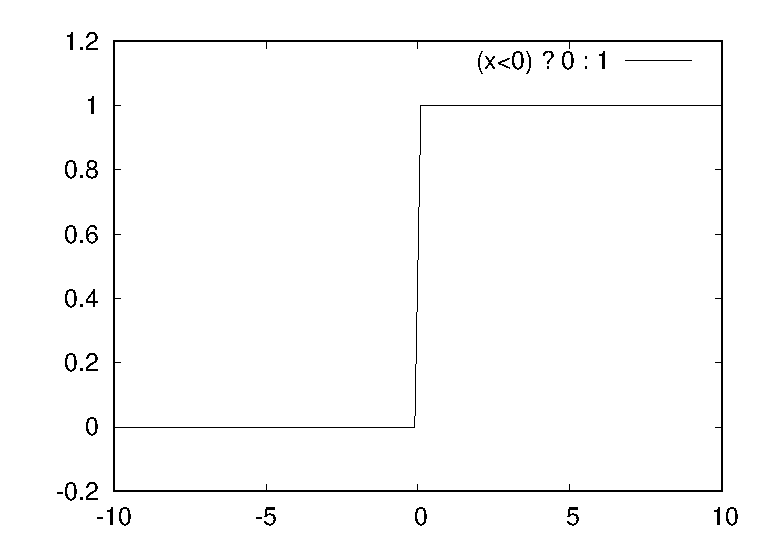
\includegraphics[width=\hsize]{ternary_operation.eps}
 \caption{三項演算子の利用}
\label{ternary}
\end{minipage}
\end{center}
\end{figure}

\section*{Appendix 4:  媒介変数の利用({\tt\bf set parametric})}
これまで紹介したものはすべて $y=f(x),z=f(x,y)$ と表せるものでした。
しかしこれだけでは表現できないものもあります。そんなとき、gnuplotでは媒介変数を利用することもできます。
\begin{terminal}
 gnuplot> {\bf set parametric}
\end{terminal}
と入力することで媒介変数モードとなります。
このとき媒介変数として認識される変数は、二次元プロットなら「t」、
三次元プロットなら「u,v」となります。
次に円・球を描く例をのせます。

円を描く(図\ref{circle})
\begin{terminal}
 gnuplot> {\bf set parametric}\\
 gnuplot> {\bf plot} cos(t),sin(t)
\end{terminal}

球を描く(図\ref{sphere})
\begin{terminal}
 gnuplot> {\bf set parametric}\\
 gnuplot> {\bf splot} sin(u)*cos(v),sin(u)*sin(v),cos(u)
\end{terminal}

\begin{figure}
 \begin{center}
  \begin{minipage}[hbtp]{0.49\textwidth}
   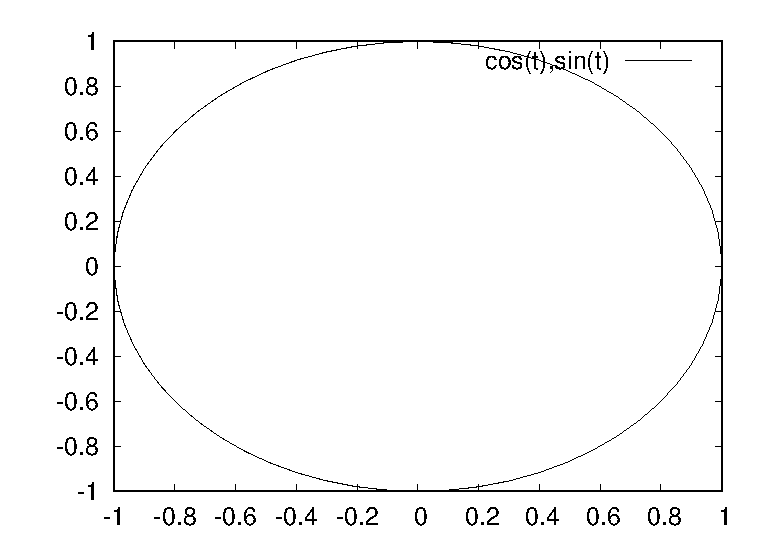
\includegraphics[width=\hsize]{circle.eps}
   \caption{媒介変数の使用(円)}
   \label{circle}
  \end{minipage}
  \begin{minipage}[hbtp]{0.49\textwidth}
   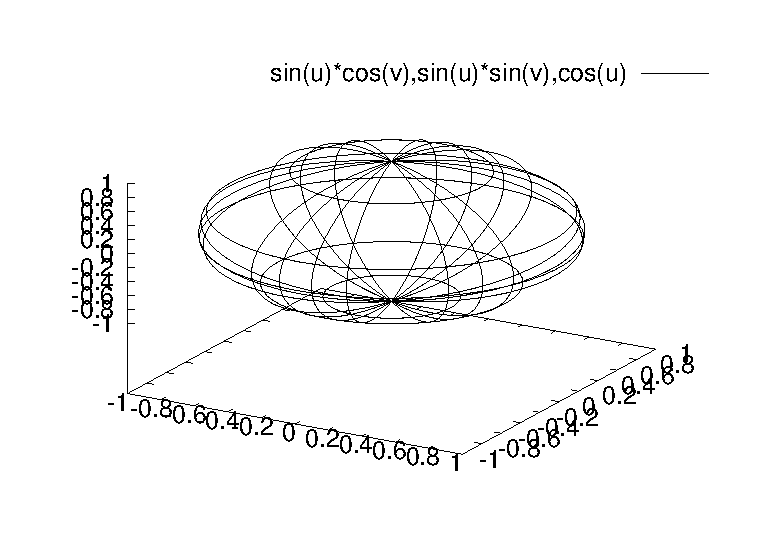
\includegraphics[width=\hsize]{sphere.eps}
   \caption{媒介変数の使用(球)}
   \label{sphere}
  \end{minipage}
 \end{center}
\end{figure}

\section*{Appendix 5:  gnuplot上でのshellコマンドの利用({\tt\bf shell, !})}
gnuplot から一時的に shell に抜けることができます。そのためには、
\begin{terminal}
 gnuplot> {\bf shell}
\end{terminal}
と打ちます。そうするとプロンプトが gnuplot 起動前のものに戻るはずです。
gnuplot に戻りたいときには{\tt\bf exit} で shell を終了して gnuplot のプロンプト
に戻ってきます。

1行だけの shell コマンドなら {\tt\bf ! command} を使って gnuplot 内から
実行することもできます。例えば
\begin{terminal}
 gnuplot> {\bf !ls}
\end{terminal}
などとやってみてください。

また、{\tt\bf pwd} と {\tt\bf cd} は gnuplot のコマンドラインからも実行
できます({\tt\bf cd}は {\tt\bf !}をつけると使えません )。
以下の例のように、ディレクトリ名は必ず引用符で括る必要がある
ことに注意してください。
\begin{terminal}
 gnuplot> {\bf cd '../'}
\end{terminal}

\section*{Appendix 6:  最小二乗フィッティング}
gnuplotの強力な機能の一つとして関数のフィッティング(当てはめ)がありま
す。パラメータを含んだ関数を用意すると、データファイルの数値に対して
適当なパラメータの数値を自動的に検索してくれます。関数は線形、非線形
を問いません。\\

例として、あるデータファイル 'linear.dat' を直線にフィッティングする
ときを考えます。まず、パラメータを含む関数$f(x)$を定義します。
関数フィッティングには{\tt\bf fit} コマンドを使います。
オプションとして検索したいパラメータ名を {\tt\bf via}に続けて与えます。

\begin{terminal}
 gnuplot> {\bf f(x) = a*x + b}\\
 gnuplot> {\bf fit f(x) 'linear.dat' via a, b}\\
 gnuplot> {\bf plot 'linear.dat'}\\
 gnuplot> {\bf replot f(x)}
\end{terminal}

収束しない場合は、大雑把に検討をつけた初期値を
手で与えてやれば上手くいく場合が多いです。
例えば、関数 $f(x)$ を定義したあとに
$a = -3$ などとして初期値を与えてから{\tt\bf fit} します。

\section*{Appendix 7:  画像の処理について(gv, Image Magick, GIMP)}
画像を処理する方法はいくつかありますが,ここでは簡単に4つほど紹介します.

\paragraph{{\tt\bf gv}}
{\tt\bf gv}はターミナル上で,
\begin{terminal}
\$ gv ***.ps
\end{terminal}
のように打つと画像がババっと表示されるコマンドです。簡単に図を確認する事ができるので今後よく使用すると思います。

(というか既に使っていますね)

\paragraph{{\tt\bf Image Magick}}
Image Magickはps, eps, jpg, png, gifなど多くの形式に対応した
画像処理ソフトです。
主に{\tt\bf display}というコマンドと
{\tt\bf convert}というコマンドを使います。

{\tt\bf display}はターミナル上で,
\begin{terminal}
\$ display ***.ps
\end{terminal}
のように打つとgvと同様に画像が表示されます。

{\tt\bf convert}は画像処理のためのコマンドです。
ターミナル上で,
\begin{terminal}
\$ convert ***.ps ***.pdf
\end{terminal}
のように打つとpsファイルがpdfファイルに変換されます。

他にも
\begin{terminal}
\$ convert -resize 80 file1 file2
\end{terminal}
と打つとfile1を80%に縮小した画像がfile2に書き込まれたり、
\begin{terminal}
\$ convert -delay 50 hoge1.gif hoge2.gif hoge3.gif hogehoge.gif
\end{terminal}
と打つとhoge1$\sim$3が0.5秒ずつ流れるgifアニメーションを作る
ことができたりします。
このconvertはかなり有用だと思いますので調べて使ってみてください。

\paragraph{{\tt\bf gimp}}
{\tt\bf gimp}はターミナル上で,
\begin{terminal}
\$ gimp ***.ps
\end{terminal}
のように打つと同様に画像が表示され,色々と手を加える事もできるコマンドです。


\newpage
\section{課題}
\begin{enumerate}
\item
\textbf{\underline{媒介変数表示}}\\
半径1の円と、$x=0$、$y=0$の直線を $-1<x<1$, $-1<y<1$の範囲で描いてください。
グラフの縦横比は1:1にしてください(Hint: {\tt\bf set size square})。

\# 提出:スクリプトファイル(kadai1.plt)とグラフ(kadai1.eps)

\item
\textbf{\underline{3次元プロット}}\\
\# 提出:練習問題2-6で作成したスクリプトファイル(kadai2.plt)とグラフ(kadai2.eps)

\item
\textbf{\underline{2軸プロット}}\\
doverの /home2/masuda2019/enshu2020/data/kadai3.dat に、本国におけるバナナの輸入量についてのデータがあります。横軸に年を取り、左の$y$軸(第一軸)を用いて総輸入量の棒グラフをプロットし、さらに右の$y$軸(第二軸)を用いて各国からの輸入量の総輸入量に対する割合(\%)をプロットしてください。

\paragraph{Hint}

\begin{terminal}
 gnuplot> {\bf set y2tics}\\
 gnuplot> {\bf p 'データ1'}\\
 gnuplot> {\bf rep 'データ2' axes x1y2}
\end{terminal}
     
\# 提出:スクリプトファイル(kadai3.plt)とグラフ(kadai3.eps)

\item
\textbf{\underline{最小二乗フィッティング}}\\
大気中に2つの等圧面があり、圧力差$\Delta p$,高度差$\Delta z$
であるとすると
\begin{equation}
 \Delta p = \rho g \Delta z \nonumber
\end{equation}
という関係が成り立ちます($\rho$:密度,$g$:重力加速度)。状態方程式より
\begin{equation}
 \rho = \frac{p}{RT} \nonumber
\end{equation}
なので(R:空気の気体定数,T:絶対温度)、温度がほぼ一定という近似のもとで積分すると
\begin{eqnarray}
 p=p_0 \exp{\left(-\frac{z}{H}\right)} \nonumber \\
 \Leftrightarrow \log{p}=\log{p_0}-\frac{z}{H} \nonumber
\end{eqnarray}
となります。
ここで$H=RT/g$をスケールハイトといい、
大気の厚さの目安として知られています。

doverの /home2/masuda2019/enshu2020/data/kadai4.dat にはラジオゾンデ観測によって得られた気圧の鉛直プロファイルが書かれています
(1行目:高度(m)、2行目:気圧(hPa)、3行目:気圧の自然対数)。
最小二乗法により傾きを求め、そこからスケールハイトを求めて
みましょう。

\paragraph{Hint}

\begin{terminal}
 gnuplot> {\bf f(x) = a*x + b} \\  
 gnuplot> {\bf plot 'kadai4.dat' using 1:3} \\
 gnuplot> {\bf fit f(x) 'kadai4.dat' using 1:3 via a, b}
\end{terminal}

\# 提出:求まった\textbf{スケールハイト}(kadai4.txt)
     + 横軸を高度、縦軸を気圧の自然対数として、観測値とフィッティングした結果の
     直線の両方をプロットしたグラフ(kadai4.eps)

\newpage
\begin{figure}[h]
 \begin{center}
  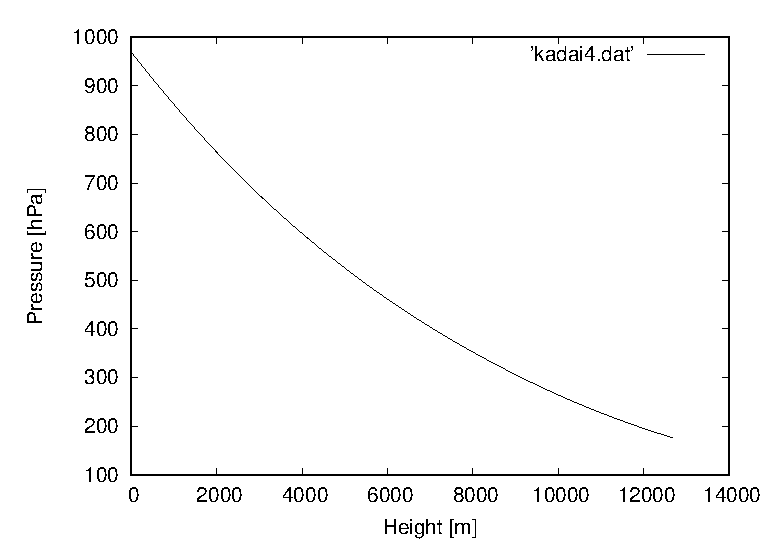
\includegraphics[width=0.6\hsize]{kadai4-1.eps}
  \caption{高度と気圧}
 \end{center}
\end{figure}

\begin{figure}[h]
 \begin{center}
  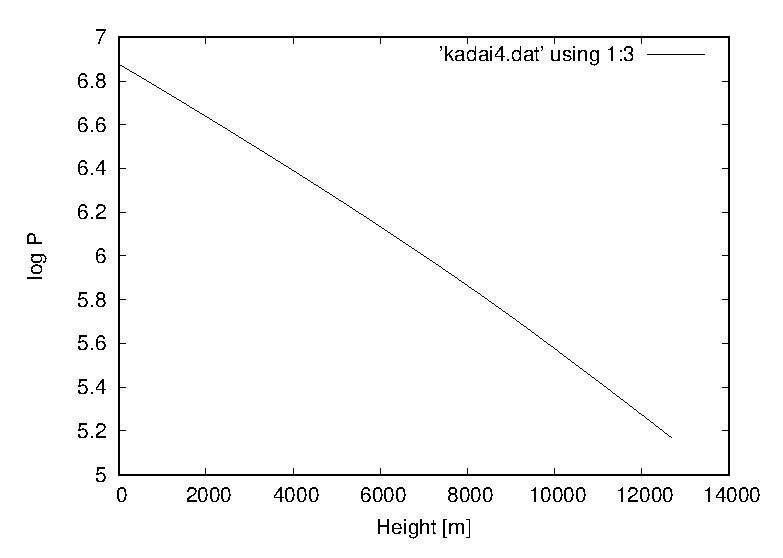
\includegraphics[width=0.6\hsize]{kadai4-2.eps}
  \caption{高度と気圧の自然対数}
 \end{center}
\end{figure}

\end{enumerate}
doverの /home2/masuda2019/enshu2020/teishutsu に s2026?? (??は自分の学生証番号の下2桁)というディレクトリを作成し、そのなかに全課題で指定されたファイル8つを置いてください。すべてのグラフには単位を明記した軸ラベル、タイトルをつけ、見やすいグラフにしてください。スクリプトファイルはloadすると一発でグラフが表示されるものとし、読みやすいように記述してください。また、提出したファイルはTAは読めるが他の学生は読めないように適切にパーミッションを設定してください。

提出期限は\textbf{5月7日(木)12時59分}とします。
\end{document}
